\documentclass[convert={density=300,size=1080x800,outext=.png}]{standalone}
\usepackage{tkz-graph}
\usetikzlibrary{arrows,positioning,shapes,shapes.multipart,patterns,mindmap,shadows}
\usepackage{xcolor}
\usepackage{helvet}
\renewcommand{\familydefault}{\sfdefault}


\begin{document}

\footnotesize
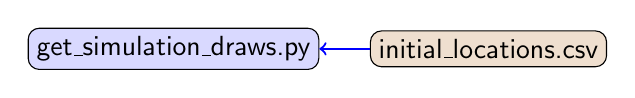
\begin{tikzpicture}[every node/.style={
    rectangle,
    rounded corners,
    inner sep=3pt,
    draw,
    fill=brown!25
}]
    \node (get_simulation_draws_py) [fill=blue!15, shift={(-4, 0)}]
    {
        get\_simulation\_draws.py
    };
    \node (initial_locations_csv) [shift={(0, 0)}]
    {
        initial\_locations.csv
    };
    \draw[->, blue, thick] (initial_locations_csv) to (get_simulation_draws_py);
\end{tikzpicture}

\end{document}